\section{Background and Design Overview}
\label{sec:bg}

This section teaches the two DNP3 transactions the paper works with, the point from which an
adversary observes them, the two features that leak, and the shape of the defended traffic we want to
produce. It uses no switch-internal names; those appear only in the implementation
(Section~\ref{sec:impl}).

\subsection{The native read transaction}
A DNP3 exchange runs between a \emph{master} (a control center) and an \emph{outstation} (a field
device; here a protective relay). To read data, the master sends a READ request, and the outstation
answers. On the wire the answer arrives as two events, shown in Fig.~\ref{fig:native}: first a TCP
segment that carries the acknowledgment (ACK) flag, then the DNP3 application response itself, which
DNP3 marks with application function code~0x81. On the SEL-751 the response is a 49-byte DNP3 frame
that fits in one TCP segment.

\begin{figure}[t]
\centering
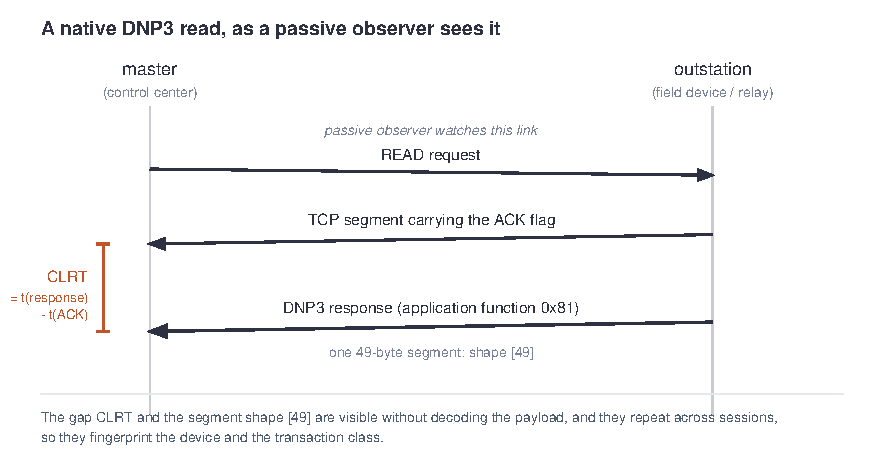
\includegraphics[width=0.98\columnwidth]{figures/fig_native}
\caption{A native read as a passive observer sees it. After the request, the outstation sends a TCP
segment carrying the ACK flag and then the DNP3 application response (function~0x81). The cross-layer
response time (CLRT) is the interval between those two packets; the response is a single 49-byte
segment, a shape we write $[49]$.}
\label{fig:native}
\end{figure}

\subsection{The native control transaction}
Control is a two-step exchange called select-before-operate. The master first sends a SELECT that
arms a control point; the outstation confirms it. The master then sends an OPERATE that actuates the
point, and the outstation echoes the command back. The two steps exist so that a stray or replayed
OPERATE with no matching SELECT cannot act.

\subsection{The observation point}
We assume a passive observer on the \emph{master-facing} link, the segment between the master and the
switch. It records TCP and IP headers, TCP segment sizes, and arrival times. It does not see the
\emph{relay-facing} link between the switch and the outstation, nor anything internal to the switch.
Fig.~\ref{fig:threat} places the observer and marks the relay-facing link as unobserved.

\begin{figure}[t]
\centering
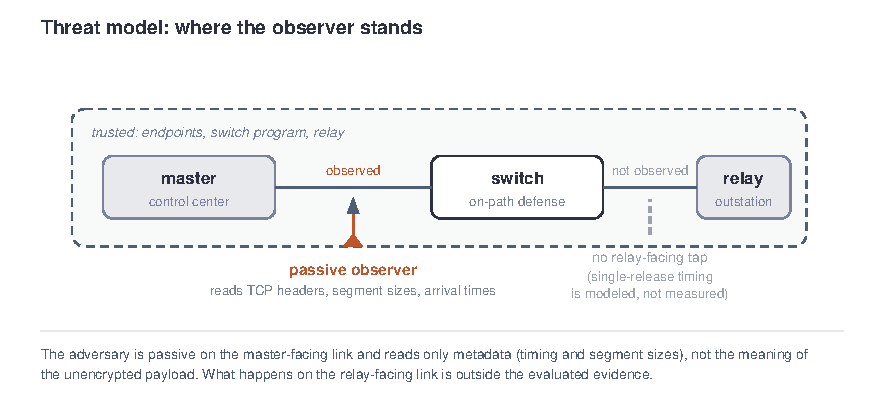
\includegraphics[width=0.98\columnwidth]{figures/fig_threat}
\caption{Threat model. The passive observer sits on the master-facing link and reads only metadata
(TCP headers, segment sizes, arrival times). The relay-facing link is not observed, so the internal
release timing of a control command is modeled, not measured.}
\label{fig:threat}
\end{figure}

\subsection{The two leaked features}
From that vantage the observer reads two features without decoding the payload. The \emph{cross-layer
response time} is the gap between the ACK-bearing segment and the DNP3 response defined above; it
reflects the outstation's internal processing. The \emph{segment shape} is the vector of TCP segment
sizes the response is delivered in ($[49]$ natively). Because the outstation is deterministic, both
features repeat across sessions, so they fingerprint the device and separate its transaction classes:
on the SEL-751 the read and select classes differ in CLRT (medians near 1.3 and 2.1~ms).

\subsection{What defended traffic should look like}
The defense produces two changes on the master-facing link, shown in Fig.~\ref{fig:shape}. It fixes
the CLRT to a single policy value, so the timing no longer separates the classes. And it fixes the
segment shape to $[28,21]$: the same 49 bytes, now delivered as two segments of 28 and 21 bytes. The
cut is placed at a boundary DNP3 already uses. A DNP3 frame is a link header followed by 16-byte data
blocks, each closed by a 2-byte CRC that the master validates; cutting between two such blocks yields
two segments that each end on an already-valid CRC, so no byte is edited and no CRC is recomputed.
Byte~28 is one such boundary. The reassembled response is still 49 bytes: the defense normalizes the
observed shape and timing, not the total length, which a full TCP reader still recovers.

\begin{figure}[t]
\centering
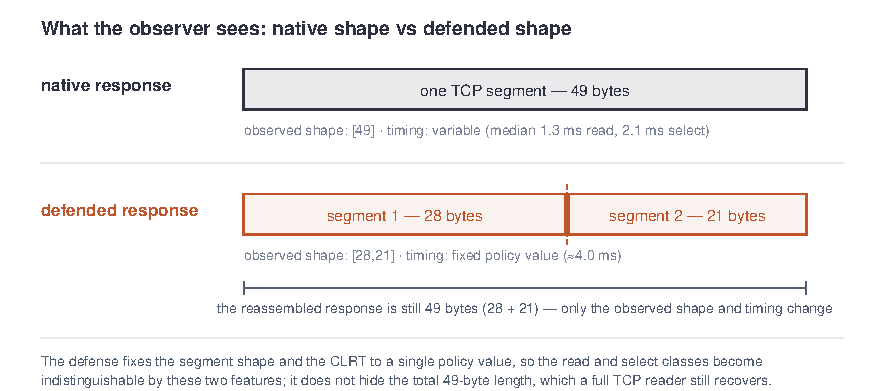
\includegraphics[width=0.98\columnwidth]{figures/fig_shape}
\caption{Native versus defended, as observed. The native response is one 49-byte segment with variable
timing; the defended response is the same 49 bytes as a fixed $[28,21]$ two-segment shape with a fixed
CLRT. The total length is unchanged.}
\label{fig:shape}
\end{figure}

\subsection{The two treatments and why they are separated}
Two treatments produce these changes. \emph{Response shaping} handles a read or select response: it
holds the acknowledgment and the response, releases each at a fixed offset from the request so the
CLRT is a constant, and splits the released response into the $[28,21]$ shape. \emph{The
control-command treatment} handles the OPERATE: it holds the command and releases it once at an
internal delay, while pinning the master-visible acknowledgment and echo to the request's arrival so
that the observable gap does not vary with the internal delay. The two treatments cannot share one
priority schedule. Response shaping keeps a set of higher-priority ``blocker'' packets draining to
time its release; if the held control command sat below them on the same schedule, those blockers
would starve it and its release would drift toward the response's release time instead of its own.
The design therefore gives the two treatments \emph{two independent scheduling lanes} inside the same
switch, as Fig.~\ref{fig:scheduler} shows; both are internal paths in one switch and one program, not
extra devices or a second pipeline.
